\chapter{Branch Coverage}

\section{Introduction}
This chapter details my effort to implement branch coverage. The structure of the chapter is largely the same as the previous chapter. However, there is a lot more detail provided on the algorithm as it is thought to be the only detailed description on the process of converting an Abstract Syntax Tree to a Control Flow Graph.

\section{Analysis}

As detailed in the literature review, branch coverage is how many conditional statements have had all possible paths executed. So for an \verb|if| statement, if it only ever evaluates to \verb|true| then the branch coverage at that vertex is 50\%. This becomes a problem when you have code such as in Figure \ref{lst:branchingExample}.If the \verb|if| statement always evaluates to true during testing, statement coverage will show as being over 99\%. However, if it ever evaluates to false then \verb|someObject| won't be initialised, and an exception will be thrown later on if somewhere else \verb|someObject| is referenced.

\begin{figure}
\centering
\begin{minipage}{.33\textwidth}
  \centering
  \lstinputlisting{code/branch_example.java}
  \caption{Some sample pseudocode}
  \label{lst:branchingExample}
\end{minipage}%
\begin{minipage}{.5\textwidth}
  \centering
  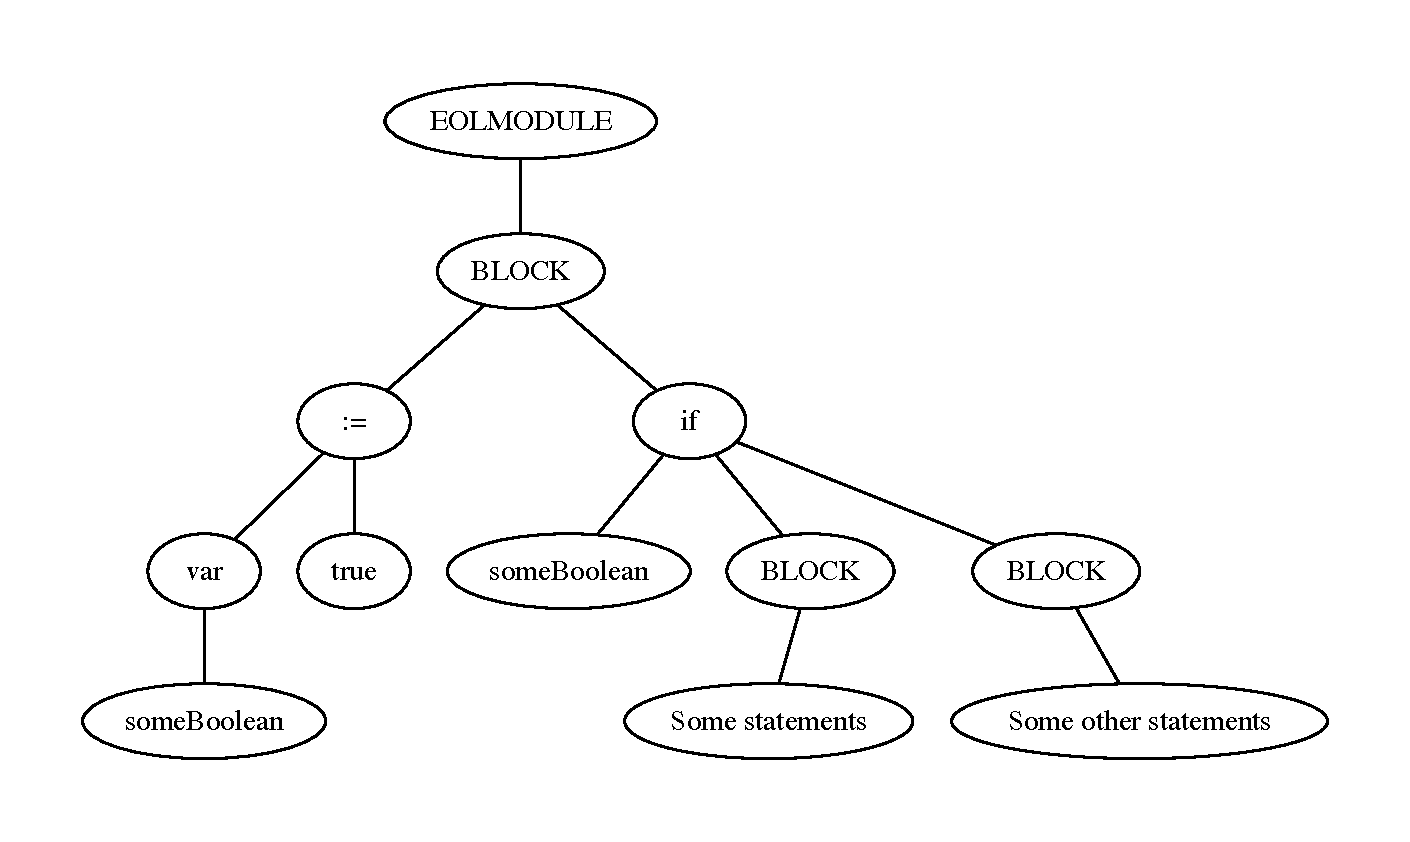
\includegraphics[scale=0.5]{figures/branchSampleAST.pdf}
  \caption{The AST of the program in Figure \ref{lst:branchingExample}}
  \label{fig:branchExampleAST}
\end{minipage}
\end{figure}

Branch coverage can counter this by looking at how many of the possible paths after all conditional statements have been executed. So in the code in Figure \ref{lst:branchingExample}, only 50\% of possible paths from that \verb|if| statement have been executed, and so the branch coverage is 50\%.

By looking at the AST (Figure \ref{fig:branchExampleAST}) of the sample code, it would appear that by counting the number of blocks below the \verb|if| vertex, we could determine how many branches in the code there are, and after execution we could see how many of those branches have been executed.

Unfortunately this approach is not perfect. The blocks only appear when curly braces are used. If just a single statement is placed under the \verb|if| statement, then the block is skipped and just a vertex for the single statement appears. So this means that the code is now more complex than it was previously thought to be. Furthermore, if statements can have children that never need to be executed, and so my algorithm would need to include details of this. If these were the only drawbacks then I would still choose this approach. However, this kind of caveat occurs for many conditional statements, and so the code that would be produced would be rather unwieldy and difficult to maintain.

The approach therefore that I have chosen to take is actually quite difficult to justify. I suggest that the AST be converted to a Control Flow Graph, at which point the branches from each vertex will be clear. A record will be made on which edges between vertices have been executed, and the total number of edges will be counted. The edges that have not been recorded will map to the branches that were not taken. The reason that this is difficult to justify is that an extensive search has not come up with any explicit instructions on how to go about generating a control flow graph from an abstract syntax tree. Furthermore, the complexities of special code for each type of statement will still apply when performing the conversion. However, some forward thinking means that the conversion from AST to CFG will be necessary when performing the path coverage because of the formula detailed in the literature review's path coverage section, and so this effort will solve two problems, and will have a quicker overall development time.

Before beginning development, a list was made of the statements that need to be included. This was done by going through the Epsilon book \citep{epsilonBook} which is a complete source of EOL syntax, but also as well by going through the EuGENia source to see which statements are actually used. The list was then loosely ordered in priority based on the number of uses within the EuGENia source. The list as as follows:

\begin{enumerate}[nolistsep]
\item I
\item Have
\item Temporarily
\item Misplaced
\item The
\item List
\item but
\item I
\item know
\item where
\item it
\item is
\end{enumerate}

For each of the identified statements, I will individually analyse how they can be converted from an AST to a CFG. For each statement a sample AST will be shown, as well as the desired CFG.

\subsection{The if statement}

\subsection{The while loop}

\begin{figure}
\centering
\begin{minipage}{.3\textwidth}
  \centering
  \lstinputlisting{code/statements/while.java}
  \caption{}
  \label{lst:whileBranch}
\end{minipage}%
\begin{minipage}{.3\textwidth}
  \centering
  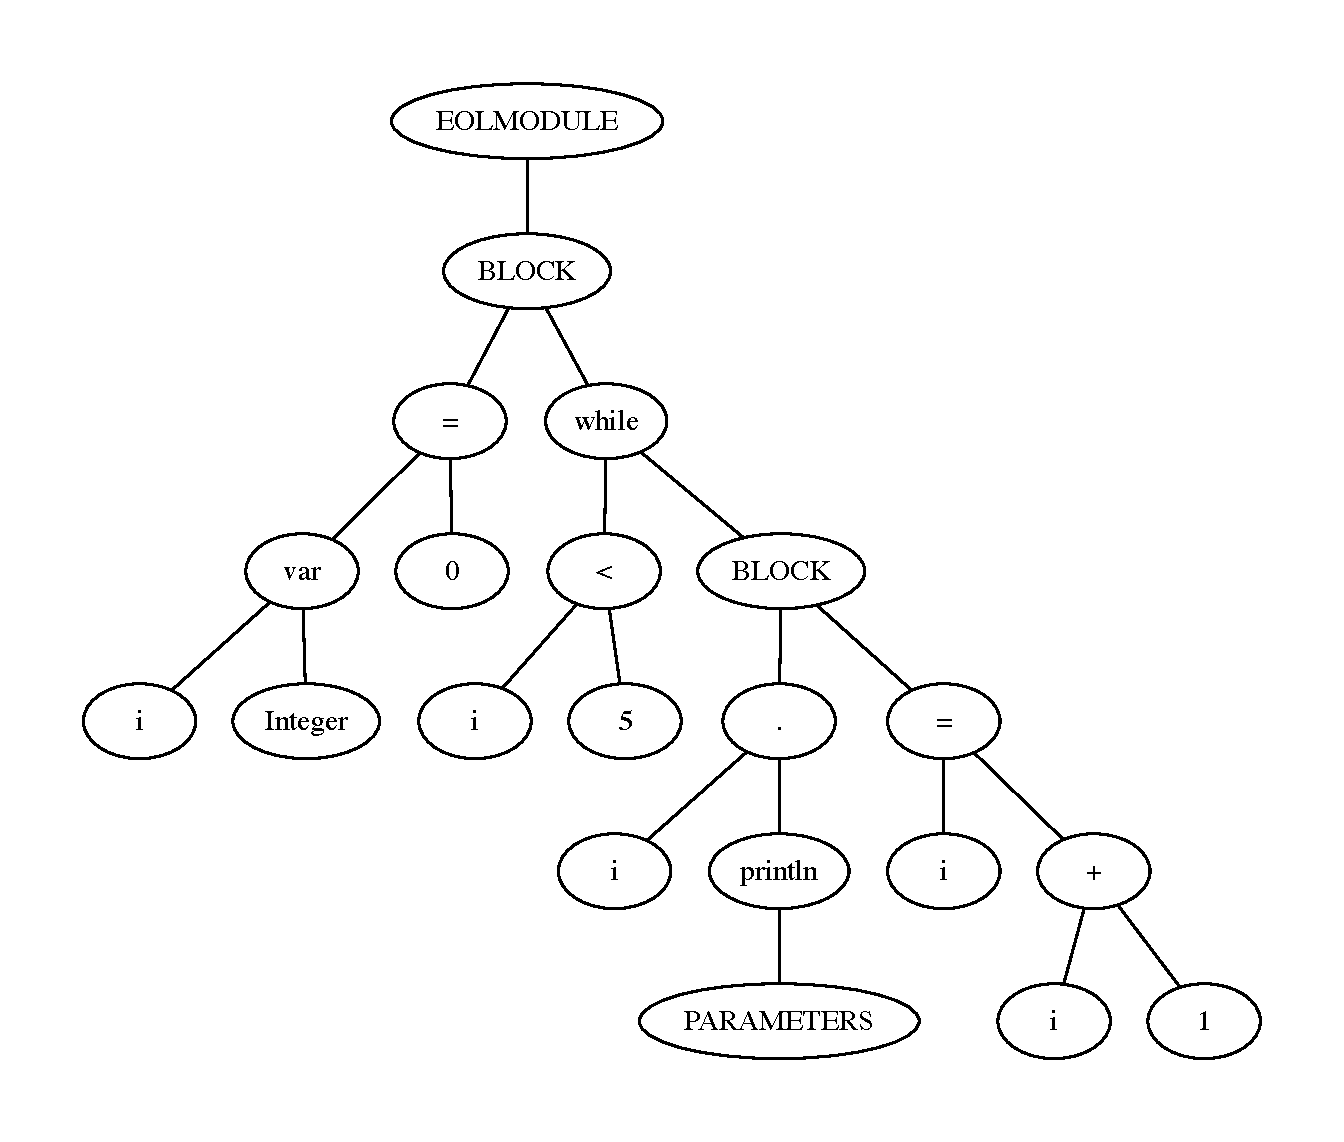
\includegraphics[width=\linewidth]{figures/statements/while_AST.pdf}
    \caption{}
  \label{fig:whileAST}
\end{minipage}
\begin{minipage}{.3\textwidth}
  \centering
  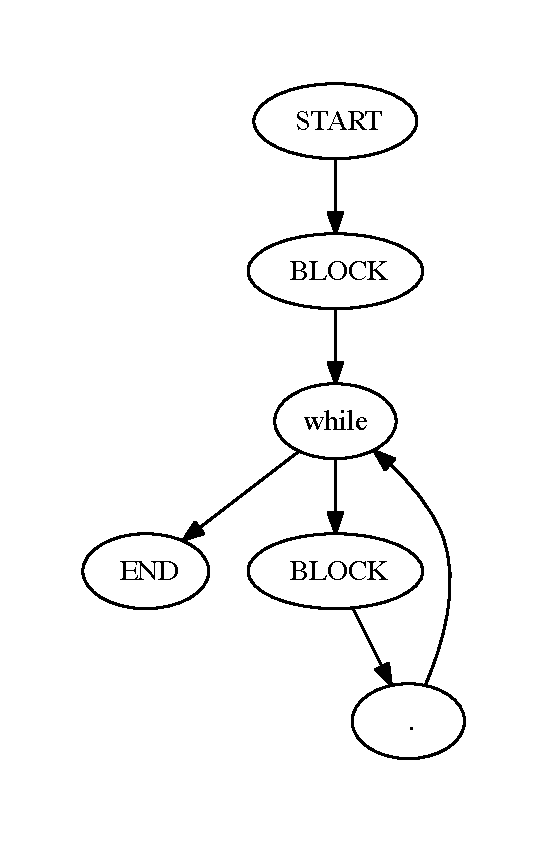
\includegraphics[scale=0.5]{figures/statements/while_CFG.pdf}
    \caption{}
  \label{fig:whileCFG}
\end{minipage}
\end{figure}